\documentclass[a4paper, 12pt, spanish]{article}

\usepackage[left=2.3cm, right= 1.8cm, top=2.5cm, bottom=2.2cm]{geometry}
\usepackage[es-tabla]{babel}
\usepackage{float}
\usepackage{tabto}
\usepackage{inconsolata}
\usepackage{graphicx}
\usepackage{wrapfig}
\usepackage{enumitem}
\usepackage{fancyhdr}
\usepackage{amsmath}
\usepackage{mathrsfs}
\usepackage{mathtools, nccmath}
\usepackage{index}
\usepackage{listings}
\usepackage{pdflscape}
\usepackage{multicol}
\usepackage{tikz}
\usepackage{marginnote}
\usepackage[format=plain,
            labelfont={it,bf},
            textfont=it, justification = centerlast]{caption}
\usetikzlibrary{calc,patterns,arrows,shapes.arrows,intersections, decorations.pathmorphing}
\usepackage[hidelinks, pdftex]{hyperref}
\usepackage[nameinlink]{cleveref}
\usepackage{subfig}
\usepackage{booktabs}
\usepackage{multirow}
\setlength{\columnsep}{1cm}
%\setlength{\columnseprule}{0.5pt}

\newcommand{\rot}{\nabla\times}

\crefname{table}{tabla}{tablas}
\Crefname{table}{Tabla}{Tablas}
\begin{document}
\pagestyle{fancy}\setcounter{page}{1}
\pagestyle{headings}
\begin{center}
\LARGE{\textbf{Propiedades Térmicas: Prácticas}} \rule{.9\textwidth}{.05cm}
\end{center}
\begin{flushright}
Alberto Peinador Veiga,\\
Universidad de Sevilla,\\
\Today
\end{flushright}

\begin{multicols}{2}
\section{Práctica 1: ciclo de histéresis.}
En la \Cref{fig:t} se representan los resultados de campo eléctrico y polarización con respecto al tiempo.
En ellos se ve como en todos los casos el campo eléctrico se mantiene independiente de la temperatura. La polarización si que tiene un respuesta diferente según la temperatura.\\
A temperatura baja la forma de la curva es muy similar a la del campo eléctrico. Se podría decir que son proporcionales, lo que concuerda con un régimen paraeléctrico. A temperaturas mayores, la polarización aumenta rápidamente en tiempos en los que el campo eléctrico es bajo hasta que llega a saturar. En el punto intermedio (\texttt{C6.DAT}) se puede percibir una combinación de ambas curvas.

\begin{figure}[H]
    \centering
    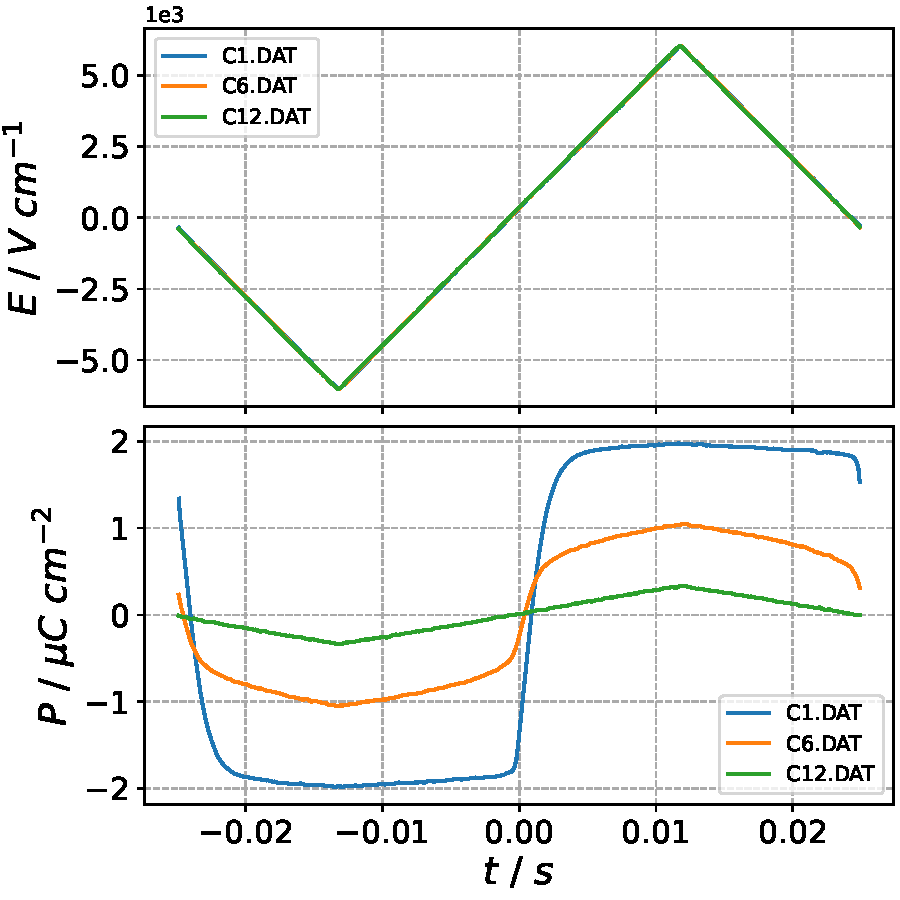
\includegraphics[width = \linewidth]{/Users/albertopeinador/Desktop/Master/termicas/E-t.pdf}
    \caption{Campo eléctrico y polarización como función del tiempo a distintas temperaturas.}\label{fig:t}
\end{figure}
La polarización remanente es la polarización cuando el campo eléctrico es nulo, mientras que el campo coercitivo es el campo eléctrico al que se anula la polarización. Para obtener estos parámetros se busca en los datos estos puntos, o en su defecto los más cercanos.

\begin{table}[H]
    \centering
    \caption{Valores de $P_r$ y $E_c$ recogidos tanto para el TGS como para LATGS, calculados tomando la media entre los tres puntos más cercanos. Los valores se presentan en con las mismas unidades que en la \Cref{fig:t}.}\label{tab:Pr_ej1}
    \begin{tabular}{cccc}\toprule
    Muestra & Región & $P_r$ & $E_c$\\ \midrule
    \multirow{2}*{TGS}& (+) & & \\
    & (-) & & \\
    \multirow{2}*{LATGS} & (+) & & \\
    & (-) &&\\ \bottomrule     
    \end{tabular}
\end{table}
%     ###################    (SUB)TABLES EXAMPLES      ###################


%\begin{table}[htpb]
%    \centering
%    \caption{Resumen de los picos observados en el espectro general.}
%    \subfloat[Fotoelectrones]{%
%        \begin{tabular}{ccc}
%			\toprule
%Elemento & Orbital & $E_B\ /\ eV$ \\ \midrule
%Na & 1s & 1070 \\
%Zn & 2p & 1020 \\
%Cu & 2p & 930 \\
%F & 1s & 683\\
%O & 1s & 531\\
%Ca & 2s & 438\\
%C&1s&284.6 \\ 
%Ar & 2p & 243\\
%Mo & 3d & 230\\
%Cu & 3s & 119\\
%Cu & 3p & 74\\
%\bottomrule
%        \end{tabular}
%        \label{tab:picos_ye}%
%    }
%    \qquad \ \qquad
%    \subfloat[Electrones Auger]{%
%        \begin{tabular}{ccc}
%            \toprule
%            Elemento & Transición & $K\ /\ eV$ \\ \midrule
%             Mo & NMV & 186 \\
%             C & KLL & 266\\
%             O & KLL & 489\\
%             F & KLL & 657\\
%             Zn & LMM & 989\\
%             Mg & KLL & 1179\\
%            \bottomrule
%        \end{tabular}
%        \label{tab:picos_auger}%
%    }
%    \label{tab:picos}
%\end{table}

%     ###################    (SUB)FIGURES EXAMPLES      ###################

%\begin{figure}[h!]
  %\centering
  %\subfloat[\label{fig:zona1A}]{%
  %  \includegraphics[width=0.49\linewidth]{Espectros/esctro_zona1}
  %}
  %\hfill
  %\subfloat[\label{fig:zona1B}]{%
  %  \includegraphics[width=0.49\linewidth]{Espectros/esctro_zona1_B}
  %}
  %\caption{Espectros con mayor resolución en la zona del pico de Zn 2p en %energía cinética (a) y binding energy (b).}
%  \label{fig:zona1}
%\end{figure}


%\bibliographystyle{my_bibstyle}
%\bibliography{biblio.bib}



\end{multicols}
\end{document}
